\documentclass[12pt,letterpaper]{article}

\usepackage[utf8]{inputenc}
\usepackage[T1]{fontenc}
\usepackage{lmodern}
\usepackage[spanish,es-noquoting]{babel}
\usepackage[left=3cm,right=2.5cm,top=2.5cm,bottom=2.5cm]{geometry}
\usepackage{graphicx}
\usepackage{booktabs}
\usepackage{longtable}
\usepackage{array}
\usepackage{xcolor}
\usepackage{listings}
\usepackage{enumitem}
\usepackage{fancyhdr}
\usepackage{titlesec}
\usepackage[hidelinks,colorlinks=false]{hyperref}
\usepackage{caption}
\usepackage{amsmath}
\usepackage{float}

\definecolor{codebg}{RGB}{245,245,245}
\definecolor{codekw}{RGB}{0,90,180}
\lstset{
  basicstyle=\ttfamily\small,
  backgroundcolor=\color{codebg},
  keywordstyle=\color{codekw}\bfseries,
  commentstyle=\itshape\color{gray},
  breaklines=true,
  frame=single,
  columns=fullflexible,
  numbers=left,
  numberstyle=\tiny\color{gray},
  language=C,
}

\pagestyle{fancy}
\fancyhf{}
\fancyhead[R]{\small Screensaver Paralelo --- Proyecto 1, Computación Paralela y Distribuida}
\fancyfoot[C]{\thepage}
\renewcommand{\headrulewidth}{0.4pt}
\setlength{\headheight}{14pt}

\setlength{\parindent}{0pt}
\setlength{\parskip}{0.6em}

\begin{document}

% ===================== CARATULA =====================
\begin{titlepage}
\begin{center}

{\large \textbf{Universidad del Valle de Guatemala}}\\[0.3cm]
{\normalsize [Facultad / Escuela --- completar según la carátula oficial del curso]}\\[2.5cm]

{\Large \textbf{Screensaver Paralelo: Dino Autojugable}}\\[0.3cm]
{\large Paralelización con OpenMP de un ciclo de simulación de partículas de clima}\\[2cm]

{\normalsize Proyecto \#1 --- Computación Paralela y Distribuida}\\[0.2cm]
{\normalsize Docente: Marlon Fuentes}\\[2cm]

{\normalsize \textbf{Integrantes:}}\\[0.2cm]
{\normalsize Mario Rocha}\\
{\normalsize [Nombre Integrante 2] --- completar}\\
{\normalsize [Nombre Integrante 3] --- completar}\\[2.5cm]

{\normalsize Semestre 2, 2026}\\
{\normalsize Guatemala, 9 de septiembre de 2026}

\end{center}
\end{titlepage}

% ===================== INDICE =====================
\tableofcontents
\newpage

% ===================== INTRODUCCION =====================
\section{Introducción}

Este informe documenta el desarrollo del Proyecto \#1 del curso de
Computación Paralela y Distribuida (UVG, semestre 2, 2026): un
\emph{screensaver} autoejecutable estilo ``Dino de Chrome'', implementado
en C con la biblioteca gráfica SDL2, cuyo componente central --- la
simulación física de partículas de clima --- se paraleliza con OpenMP.

El objetivo del proyecto no es únicamente producir una animación visual,
sino aplicar de forma práctica los conceptos de paralelización con
memoria compartida vistos en el curso: identificar qué parte de un
programa secuencial es paralelizable, aplicar el método PCAM
(Partición, Comunicación, Aglomeración, Mapeo) para diseñar su versión
paralela, implementarla con OpenMP, y medir su desempeño real en
términos de \emph{speedup} y eficiencia frente a la versión secuencial.

El documento se organiza así: la sección de antecedentes resume los
conceptos teóricos usados (OpenMP, PCAM, speedup y eficiencia, ley de
Amdahl); el cuerpo describe el diseño del screensaver, la arquitectura
del código compartido entre las versiones secuencial y paralela, la
estrategia de paralelización aplicada y los resultados medidos; y las
conclusiones resumen los hallazgos y su relación con la teoría. Los
anexos --- diagrama de flujo, catálogo de funciones y bitácora de
pruebas --- se incluyen como apéndice con el material de soporte.

% ===================== ANTECEDENTES =====================
\section{Antecedentes}

\subsection{OpenMP}

OpenMP es una interfaz de programación de aplicaciones (API) para
programación paralela con memoria compartida en C, C++ y Fortran,
mantenida por el OpenMP Architecture Review Board. Se basa en un modelo
de ejecución \emph{fork-join}: un hilo maestro ejecuta el programa de
forma secuencial hasta encontrar una directiva de compilador (un
\texttt{\#pragma omp}) que abre una región paralela, momento en el que se
crea un equipo de hilos que ejecutan el trabajo repartido entre ellos
hasta un punto de sincronización implícito al cerrar la región, tras el
cual el hilo maestro continúa solo.\footnote{OpenMP Architecture Review
Board. \emph{OpenMP Application Programming Interface, Version 5.2}.
2021. Disponible en \url{https://www.openmp.org}.} Esta característica es
justamente la que permite paralelizar un \texttt{for} secuencial con una
sola línea (\texttt{\#pragma omp parallel for}) sin reescribir la lógica
interna del ciclo, siempre que las iteraciones sean independientes entre
sí.

Para acumular un valor entre iteraciones sin condiciones de carrera ---
como un contador que varios hilos incrementan---, OpenMP ofrece la
cláusula \texttt{reduction}, que le da a cada hilo una copia privada de
la variable, la inicializa según el operador indicado, y combina todas
las copias en la variable original al finalizar la región paralela. Esto
evita usar una sección crítica (\texttt{\#pragma omp critical}) que
serializaría esa parte del ciclo y anularía buena parte del beneficio de
paralelizar.

\subsection{El método PCAM}

PCAM es una metodología de diseño de programas paralelos propuesta por
Ian Foster, organizada en cuatro etapas: \textbf{Partición}
(descomponer el problema en tareas lo más pequeñas e independientes
posible), \textbf{Comunicación} (identificar qué datos deben
intercambiarse entre tareas), \textbf{Aglomeración} (agrupar tareas
pequeñas en unidades más grandes para reducir el overhead de
comunicación/sincronización) y \textbf{Mapeo} (asignar las tareas
agrupadas a los procesadores o hilos disponibles).\footnote{Foster, I.
\emph{Designing and Building Parallel Programs}. Addison-Wesley, 1995.
Disponible en \url{https://www.mcs.anl.gov/~itf/dbpp/}.} La sección
\ref{sec:pcam} de este informe aplica explícitamente estas cuatro etapas
al diseño de \texttt{particles\_update()}.

\subsection{Speedup, eficiencia y la ley de Amdahl}

El \emph{speedup} de una versión paralela con $p$ procesadores/hilos se
define como $S_p = T_1 / T_p$, donde $T_1$ es el tiempo de la versión
secuencial y $T_p$ el de la versión paralela con $p$ hilos; la
\emph{eficiencia} es $E_p = S_p / p$, y mide qué tan bien se aprovecha
cada hilo adicional (1.0 sería aprovechamiento
perfecto).\footnote{Grama, A., Gupta, A., Karypis, G., \& Kumar, V.
\emph{Introduction to Parallel Computing} (2.\textsuperscript{a} ed.).
Addison-Wesley, 2003.} Gene Amdahl formalizó en 1967 la idea de que el
speedup máximo alcanzable está acotado por la fracción del programa que
\emph{no} se puede paralelizar: si esa fracción secuencial es pequeña
pero fija, agregar más procesadores tiene rendimientos cada vez menores
y en algún punto el overhead de coordinar más hilos puede superar la
ganancia.\footnote{Amdahl, G. M. ``Validity of the single processor
approach to achieving large scale computing capabilities''. \emph{AFIPS
Conference Proceedings}, vol.\ 30, 1967, pp.\ 483--485.} Este proyecto
observa ese efecto directamente: como se detalla en la
sección~\ref{sec:resultados}, el \emph{speedup} deja de crecer (e incluso
empeora) al pasar de 4 a 8 hilos, precisamente porque el trabajo por hilo
se vuelve pequeño frente al overhead fijo de sincronización por frame.

% ===================== CUERPO =====================
\section{Diseño e implementación}

\subsection{Descripción del screensaver}

El screensaver dibuja un dinosaurio que salta obstáculos de forma
autónoma (regla determinista de distancia, sin inteligencia artificial),
sobre un ciclo de día/noche y estaciones (primavera, verano, otoño,
invierno) que cambian la paleta de color de la escena mediante
interpolación e integran una componente trigonométrica
(\texttt{sinf()} sobre el tiempo transcurrido). El parámetro requerido
por la rúbrica del curso es \texttt{N}: la cantidad de partículas de
clima (lluvia, nieve u hojas según la estación) que caen con física real
--- gravedad constante más viento lateral sinusoidal --- y rebotan en los
bordes laterales del lienzo. El lienzo es configurable por línea de
comandos con un mínimo de 640$\times$480 px, cumpliendo el requisito
mínimo del enunciado. La actualización de esas \texttt{N} partículas por
frame es, deliberadamente, la única parte del programa que se mide y
paraleliza --- el resto (lógica del dino, obstáculos, render) se mantiene
simple e intencionalmente secuencial para concentrar el esfuerzo de
paralelización donde realmente hay trabajo independiente y repetitivo.

\subsection{Arquitectura compartida}

Las versiones secuencial (\texttt{screensaver\_seq}) y paralela
(\texttt{screensaver\_par}) comparten prácticamente todo el código, en
\texttt{src/common/}: parseo de argumentos, física de una partícula
individual (\texttt{particle\_step}), lógica del dino y los obstáculos,
cálculo de la paleta día/noche/estación, y el render con SDL2. La única
diferencia entre binarios es la función \texttt{particles\_update()},
inyectada como puntero a función (\texttt{ParticleUpdateFn}) al loop
principal compartido \texttt{run\_app()} (\texttt{src/common/app.c}):

\begin{lstlisting}[language=C,caption={Firma compartida entre la versión seq y par (include/app.h)}]
typedef int (*ParticleUpdateFn)(Particle *particles, int n,
                                 const SimState *state, float dt);
int run_app(const Config *cfg, ParticleUpdateFn update_fn);
\end{lstlisting}

\texttt{run\_app()} soporta dos modos: interactivo (ventana SDL, loop
hasta cerrar o alcanzar \texttt{--frames}) y \texttt{--benchmark}
(headless, sin SDL, corre exactamente \texttt{--frames} pasos y mide solo
el tiempo del loop de partículas). El modo benchmark es el que se usó
para todas las mediciones de la sección~\ref{sec:resultados} y del
Anexo~3, porque aísla la sección paralelizada del resto del programa
(que nunca se paraleliza y no debe contaminar la medición).

\subsection{Aplicación del método PCAM}
\label{sec:pcam}

\begin{description}[leftmargin=2em,style=nextline]
\item[Partición] Cada partícula de clima es una tarea independiente: su
próximo estado (\texttt{x, y, vx, vy}) depende únicamente de su propio
estado actual y de \texttt{SimState} (de solo lectura), nunca del estado
de otra partícula --- no hay colisiones entre partículas por diseño. Esto
da una partición natural de grano fino: una tarea por partícula, hasta
\texttt{N} tareas totalmente independientes por frame.
\item[Comunicación] Es mínima: cada tarea solo lee \texttt{SimState}
(compartido, de solo lectura, sin necesidad de proteger) y escribe
únicamente su propio elemento del arreglo \texttt{particles[i]}. El único
dato realmente compartido \emph{en escritura} es el contador de
partículas recicladas en el frame (\texttt{respawned}).
\item[Aglomeración] Agrupar cada partícula en su propia tarea de sistema
operativo sería absurdo (miles de hilos por frame). En vez de eso,
OpenMP con \texttt{schedule(static)} agrupa las \texttt{N} partículas en
bloques contiguos, uno por hilo disponible --- la aglomeración la decide
el \emph{runtime} de OpenMP, no el código de la aplicación.
\item[Mapeo] \texttt{\#pragma omp parallel for} mapea cada bloque
aglomerado a un hilo del equipo creado por OpenMP; el número de hilos lo
decide el sistema operativo por default, o el usuario vía \texttt{--threads
N} (que llama \texttt{omp\_set\_num\_threads()} antes de correr el loop).
\end{description}

\subsection{Implementación: secuencial vs. paralela}

\begin{lstlisting}[language=C,caption={Version secuencial (src/seq/particle\_update.c)}]
int particles_update(Particle *particles, int n,
                      const SimState *state, float dt) {
    int respawned = 0;
    for (int i = 0; i < n; i++) {
        if (particle_step(&particles[i], state, dt)) {
            respawned++;
        }
    }
    return respawned;
}
\end{lstlisting}

\begin{lstlisting}[language=C,caption={Version paralela con OpenMP (src/par/particle\_update.c)}]
int particles_update(Particle *particles, int n,
                      const SimState *state, float dt) {
    int respawned = 0;

    #pragma omp parallel for schedule(static) reduction(+:respawned)
    for (int i = 0; i < n; i++) {
        if (particle_step(&particles[i], state, dt)) {
            respawned++;
        }
    }
    return respawned;
}
\end{lstlisting}

La única diferencia de código es la directiva \texttt{\#pragma omp
parallel for schedule(static) reduction(+:respawned)}: no hace falta
ningún \texttt{lock} ni sección crítica explícita porque (a) las
partículas no comparten estado entre sí, y (b) cada partícula lleva su
propio generador de números aleatorios (\texttt{rand\_r} con
\texttt{rng\_state} propio, sembrado con un multiplicador tipo hash de
Knuth por índice) --- así que tampoco hay una semilla global que
sincronizar entre hilos, un problema común al paralelizar código que
depende de \texttt{rand()} clásico. El mecanismo de sincronía de esta
versión es exclusivamente la cláusula \texttt{reduction}, que combina el
acumulador local de \texttt{respawned} de cada hilo al cerrar la región
paralela.

Programación defensiva: \texttt{parse\_args()} valida tipos (enteros bien
formados vía \texttt{strtol}), rangos (\texttt{n>0}, lienzo mínimo
640$\times$480, \texttt{fps>0}, \texttt{frames>=0}, \texttt{threads>=0})
y una regla cruzada (\texttt{--benchmark} exige \texttt{--frames>0}
para que la medición sea reproducible), todo antes de reservar memoria o
inicializar SDL; \texttt{particles\_create()} revisa el retorno de
\texttt{malloc()}; y todas las rutas de inicialización de SDL (ventana,
renderer) revisan su valor de retorno y liberan lo ya reservado antes de
salir con código de error.

\subsection{Metodología de pruebas}

Las mediciones se hicieron con el modo \texttt{--benchmark} de ambos
binarios en la misma máquina (procesador Apple Silicon, 8 núcleos
lógicos), corriendo 300 frames por medición, 10 repeticiones por cada
combinación de $N \in \{500, 2000, 8000, 20000, 50000\}$ y, en la versión
paralela, hilos $\in \{1, 2, 4, 8\}$ --- 250 mediciones en total. El
detalle completo, la captura de la corrida y el análisis están en el
Anexo~3 (sección~\ref{anexo3}).

\subsection{Resultados}
\label{sec:resultados}

\begin{table}[H]
\centering
\caption{Speedup y eficiencia promedio por combinación (N, hilos)}
\begin{tabular}{rrrrr}
\toprule
N & Hilos & T. secuencial (ms) & T. paralelo (ms) & Speedup (eficiencia) \\
\midrule
8000   & 4 & 14.531 & 6.077  & 2.39 (0.60) \\
20000  & 4 & 36.819 & 12.367 & 2.98 (0.74) \\
50000  & 4 & 93.322 & 28.305 & \textbf{3.30 (0.82)} \\
50000  & 8 & 93.322 & 37.414 & 2.49 (0.31) \\
500    & 8 & 0.974  & 9.921  & 0.10 (0.01) \\
\bottomrule
\end{tabular}
\end{table}

\begin{figure}[H]
\centering
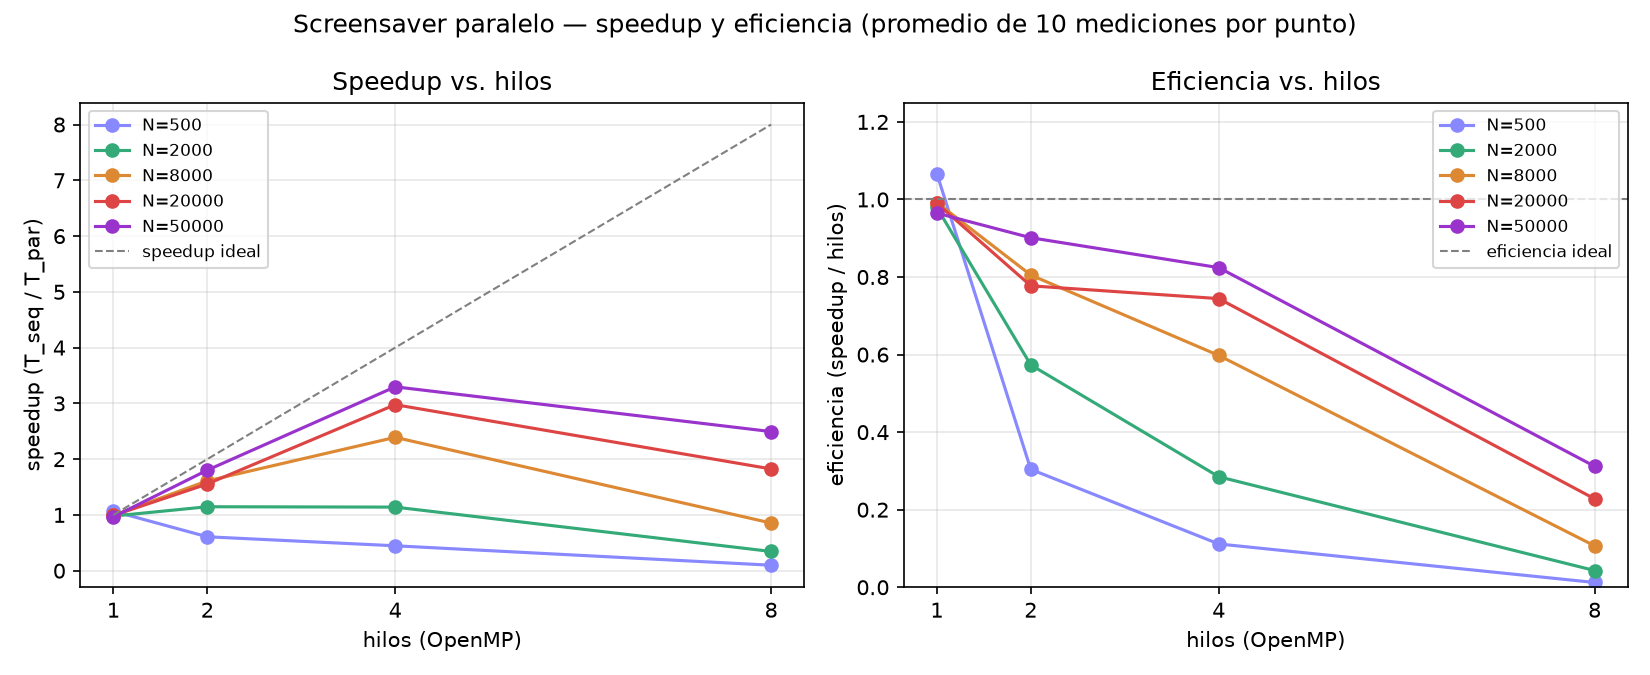
\includegraphics[width=0.95\textwidth,height=0.8\textheight,keepaspectratio]{img/anexo3_grafico_speedup_eficiencia.png}
\caption{Speedup y eficiencia medidos vs. número de hilos, por tamaño de N}
\end{figure}

El mejor resultado medido es un \textbf{speedup de 3.30x con 4 hilos y
N=50000} (eficiencia 0.82). Con \texttt{N} pequeño (500) el paralelo es
más lento que el secuencial: el overhead de OpenMP de coordinar hilos en
cada uno de los 300 \texttt{fork-join} por frame supera el trabajo real
cuando hay pocas partículas. Y en todos los tamaños de \texttt{N}
probados, \textbf{8 hilos rinde peor que 4} --- consistente con la
sección de antecedentes sobre la ley de Amdahl: el overhead fijo por
frame pesa proporcionalmente más cuantos más hilos compiten por
coordinarse, y en un chip con núcleos de rendimiento y eficiencia
heterogéneos, forzar 8 hilos reparte trabajo también sobre núcleos más
lentos. El análisis completo, con la tabla de las 20 combinaciones
medidas, está en el Anexo~3.

Se verificó además que paralelizar no altera el resultado de la
simulación: con semilla fija (\texttt{--seed 12345}, N=8000), la
versión secuencial y la paralela con 1, 4 y 8 hilos reciclan exactamente
\textbf{26144} partículas en 300 frames --- confirmando que
\texttt{reduction(+:respawned)} combina los contadores sin perder ni
duplicar eventos, y que el orden de procesamiento entre hilos no afecta
el resultado (ver Anexo~3).

% ===================== CONCLUSIONES =====================
\section{Conclusiones}

\begin{enumerate}
\item Paralelizar con OpenMP el loop de actualización de partículas fue
directo porque el problema tiene una partición natural de grano fino
(partículas independientes) con comunicación mínima (solo un contador
compartido), lo que permitió resolverlo con una sola directiva
\texttt{\#pragma omp parallel for} y una \texttt{reduction}, sin
necesidad de locks explícitos.
\item El speedup obtenido depende fuertemente de \texttt{N}: solo se
observa una ganancia real (hasta 3.30x) cuando hay suficiente trabajo por
frame para amortizar el overhead fijo de crear/sincronizar hilos; con
pocas partículas, paralelizar activamente perjudica el desempeño.
\item Más hilos no es necesariamente mejor: 4 hilos superó consistentemente
a 8 en esta máquina, lo que confirma en la práctica la intuición de la
ley de Amdahl y sugiere que la elección del número de hilos debe basarse
en mediciones, no asumirse igual al máximo de núcleos disponibles.
\item Se verificó que la paralelización no introdujo condiciones de
carrera: con semilla fija, el resultado de la simulación (partículas
recicladas) es idéntico entre la versión secuencial y la paralela, en
cualquier número de hilos probado.
\end{enumerate}

\subsection*{Recomendaciones}

\begin{itemize}
\item Para trabajo futuro, valdría la pena medir con
\texttt{schedule(dynamic)} en vez de \texttt{schedule(static)} para ver
si compensa mejor el desbalance entre núcleos de rendimiento y
eficiencia del chip usado.
\item Repetir las mediciones en una máquina con núcleos homogéneos
(p.\ ej.\ un servidor Linux) ayudaría a aislar si la caída de eficiencia
a 8 hilos es overhead de OpenMP puro o un efecto específico de la
heterogeneidad de núcleos de este equipo.
\end{itemize}

\newpage
% ===================== APENDICE =====================
\appendix
\section{Apéndice: material suplementario}

\subsection{Anexo 1 --- Diagrama de flujo}

\begin{figure}[H]
\centering
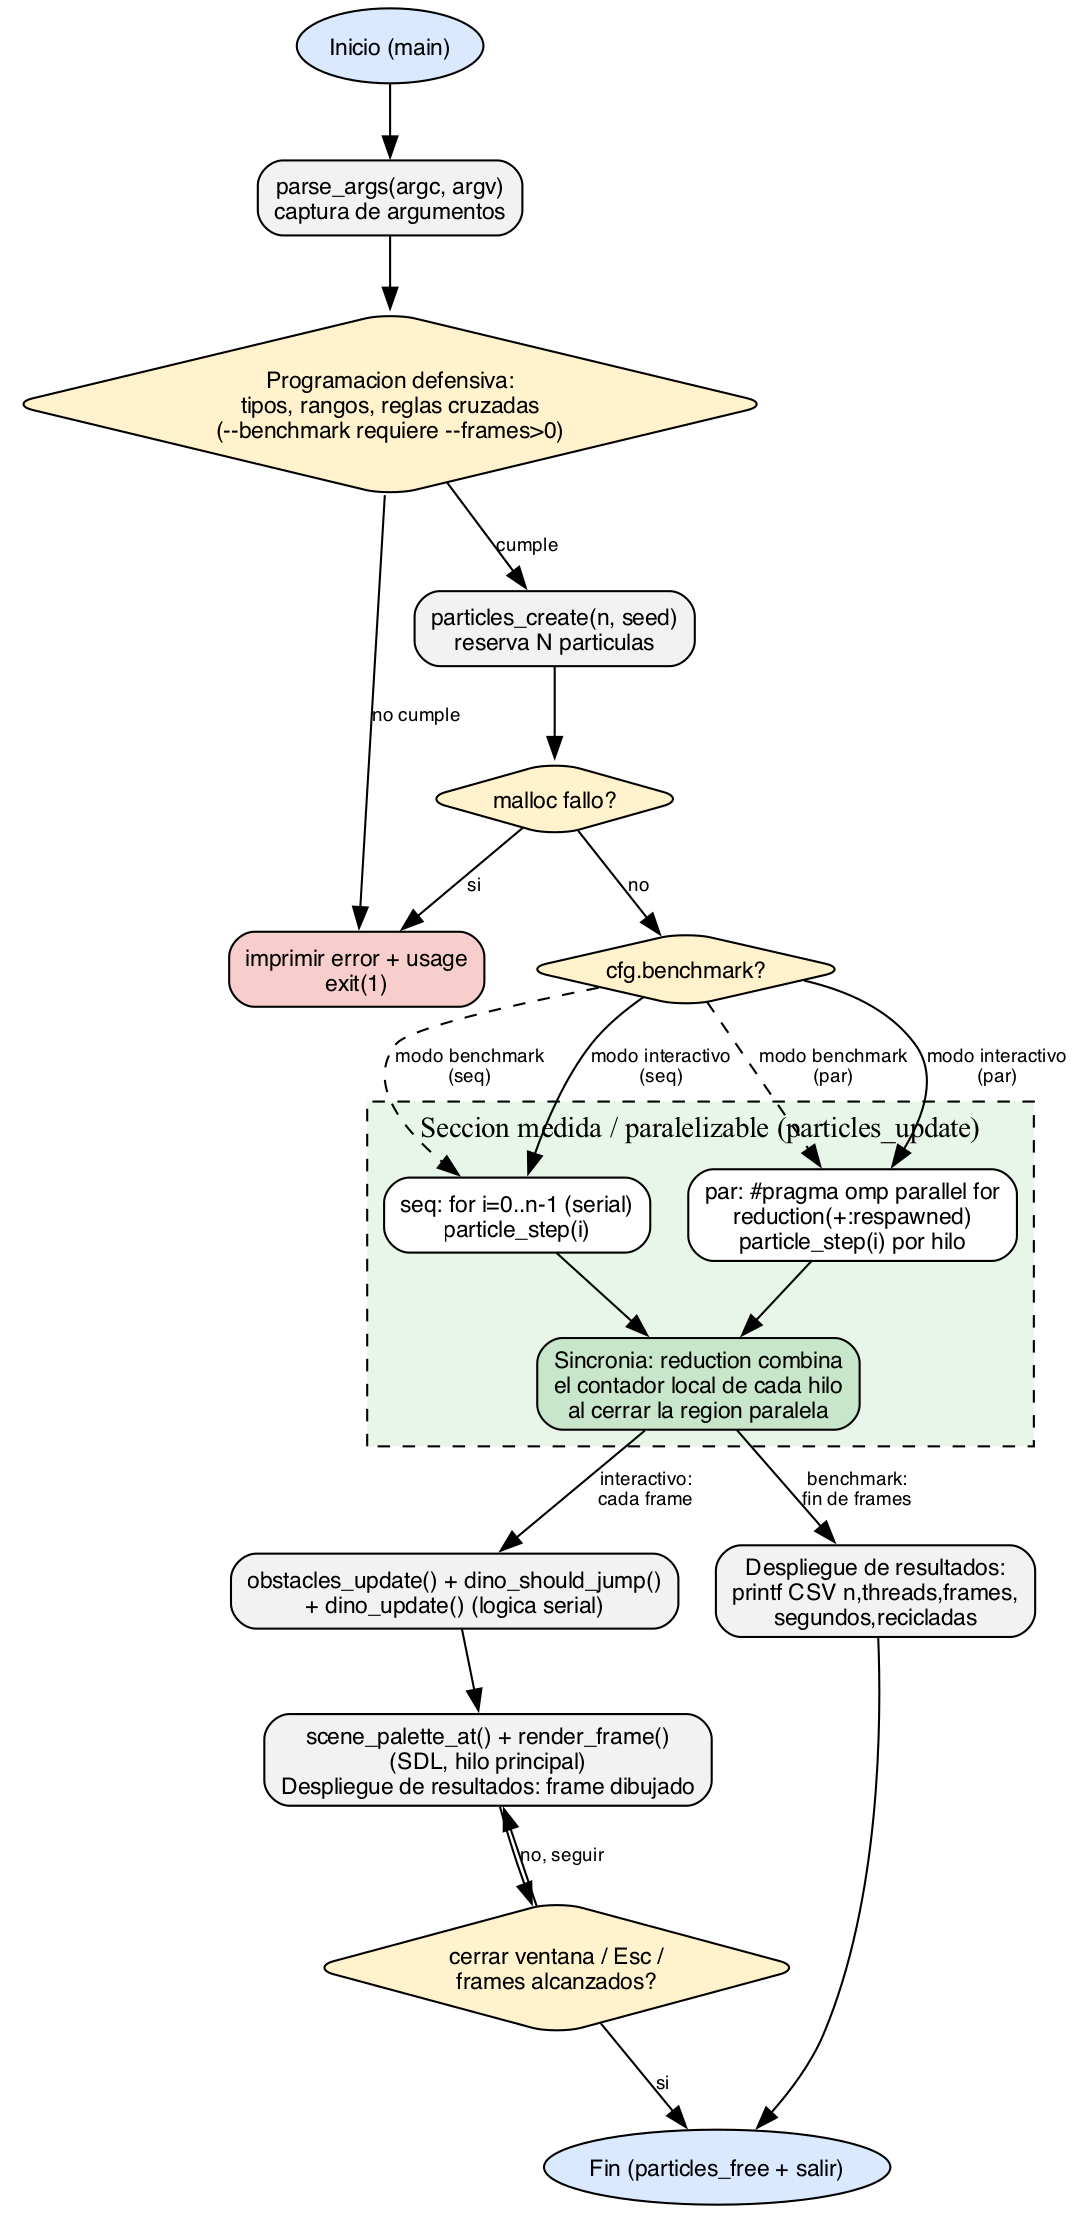
\includegraphics[width=0.85\textwidth,height=0.82\textheight,keepaspectratio]{img/anexo1_diagrama_flujo.png}
\caption{Diagrama de flujo del programa (aplica a \texttt{screensaver\_seq} y \texttt{screensaver\_par})}
\end{figure}

La versión detallada de este diagrama (con todas las ramas de validación
defensiva) está en \texttt{docs/anexo1\_diagrama\_flujo.md} del
repositorio.

\subsection{Anexo 2 --- Catálogo de funciones}

El catálogo completo de funciones del proyecto (entradas, salidas y
descripción de cada una, incluyendo las funciones \texttt{static}) está
en \texttt{docs/anexo2\_catalogo\_funciones.md} del repositorio, por su
extensión no se transcribe aquí completo. Resumen de las funciones
centrales para la paralelización:

\begin{center}
\begin{tabular}{p{3.8cm}p{4.5cm}p{5.5cm}}
\toprule
Función & Entradas / Salidas & Descripción \\
\midrule
\texttt{particle\_step} &
Entra: \texttt{Particle*}, \texttt{SimState*}, \texttt{dt}.
Sale: \texttt{bool} (¿se recicló?). &
Física de una partícula: viento sinusoidal + gravedad, rebote en
bordes, reciclaje al salir por abajo. Unidad de trabajo independiente
paralelizada. \\
\addlinespace
\texttt{particles\_update} (seq) &
Entra: arreglo de \texttt{N} partículas, \texttt{SimState*}, \texttt{dt}.
Sale: \texttt{int} partículas recicladas. &
\texttt{for} secuencial que llama \texttt{particle\_step} por cada
partícula. \\
\addlinespace
\texttt{particles\_update} (par) &
Misma firma que la versión seq. &
Igual, pero con \texttt{\#pragma omp parallel for schedule(static)
reduction(+:respawned)}. \\
\bottomrule
\end{tabular}
\end{center}

\subsection{Anexo 3 --- Bitácora de pruebas}
\label{anexo3}

\subsubsection*{Captura de la corrida de benchmarks}

\begin{figure}[H]
\centering
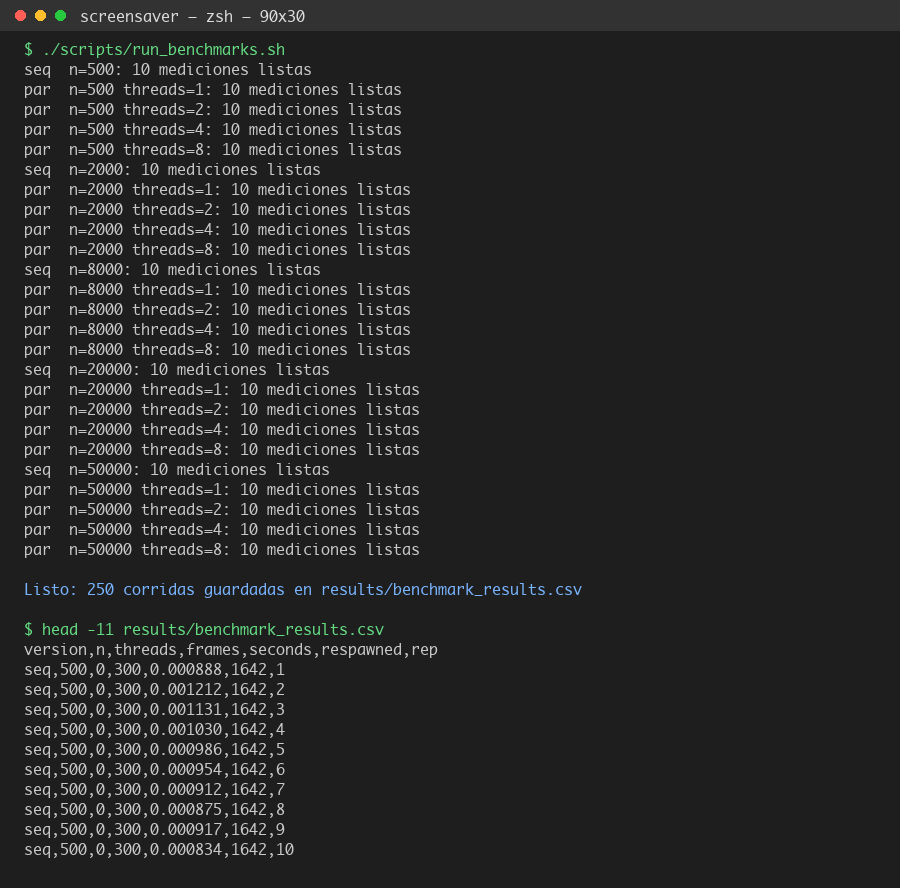
\includegraphics[width=0.85\textwidth,height=0.8\textheight,keepaspectratio]{img/anexo3_captura_mediciones.png}
\caption{Corrida real de \texttt{scripts/run\_benchmarks.sh} y primeras filas del CSV crudo generado (250 mediciones, 10 repeticiones por combinación de N y número de hilos)}
\end{figure}

\subsubsection*{Tabla completa de resultados (promedio de 10 mediciones por fila)}

\begin{longtable}{rrrrrr}
\toprule
N & Hilos & T. secuencial (ms) & T. paralelo (ms) & Speedup & Eficiencia \\
\midrule
\endhead
500   & 1 & 0.974  & 0.913  & 1.07 & 1.07 \\
500   & 2 & 0.974  & 1.602  & 0.61 & 0.30 \\
500   & 4 & 0.974  & 2.182  & 0.45 & 0.11 \\
500   & 8 & 0.974  & 9.921  & 0.10 & 0.01 \\
2000  & 1 & 3.432  & 3.505  & 0.98 & 0.98 \\
2000  & 2 & 3.432  & 2.994  & 1.15 & 0.57 \\
2000  & 4 & 3.432  & 3.011  & 1.14 & 0.29 \\
2000  & 8 & 3.432  & 9.958  & 0.34 & 0.04 \\
8000  & 1 & 14.531 & 14.648 & 0.99 & 0.99 \\
8000  & 2 & 14.531 & 9.025  & 1.61 & 0.81 \\
8000  & 4 & 14.531 & 6.077  & 2.39 & 0.60 \\
8000  & 8 & 14.531 & 17.006 & 0.85 & 0.11 \\
20000 & 1 & 36.819 & 37.195 & 0.99 & 0.99 \\
20000 & 2 & 36.819 & 23.684 & 1.55 & 0.78 \\
20000 & 4 & 36.819 & 12.367 & 2.98 & 0.74 \\
20000 & 8 & 36.819 & 20.182 & 1.82 & 0.23 \\
50000 & 1 & 93.322 & 96.725 & 0.96 & 0.96 \\
50000 & 2 & 93.322 & 51.770 & 1.80 & 0.90 \\
50000 & 4 & 93.322 & 28.305 & 3.30 & 0.82 \\
50000 & 8 & 93.322 & 37.414 & 2.49 & 0.31 \\
\bottomrule
\end{longtable}

Datos crudos completos (250 filas, sin promediar):
\texttt{results/benchmark\_results.csv}. Resumen promediado:
\texttt{results/benchmark\_summary.csv}. Script usado:
\texttt{scripts/run\_benchmarks.sh}.

\subsubsection*{Verificación de corrección (semilla fija)}

Con \texttt{--seed 12345}, N=8000, 300 frames:

\begin{lstlisting}[language=bash,caption={Verificación: mismo resultado de simulación en todos los binarios/hilos}]
seq              (1 hilo, serial): 26144 particulas recicladas
par --threads 1:                   26144 particulas recicladas
par --threads 4:                   26144 particulas recicladas
par --threads 8:                   26144 particulas recicladas
\end{lstlisting}

\subsubsection*{Análisis}

Ver el análisis completo, con la explicación de por qué N chico perjudica
el paralelo y por qué 8 hilos rinde peor que 4, en
\texttt{docs/anexo3\_bitacora\_pruebas.md} y en la
sección~\ref{sec:resultados} de este informe.

% ===================== REFERENCIAS =====================
\newpage
\section*{Referencias bibliográficas}
\addcontentsline{toc}{section}{Referencias bibliográficas}

\begin{enumerate}
\item Amdahl, G. M. ``Validity of the single processor approach to
achieving large scale computing capabilities''. \emph{AFIPS Conference
Proceedings}, vol.\ 30, 1967, pp.\ 483--485.
\item Foster, I. \emph{Designing and Building Parallel Programs}.
Addison-Wesley, 1995. \url{https://www.mcs.anl.gov/~itf/dbpp/}.
\item Grama, A., Gupta, A., Karypis, G., \& Kumar, V. \emph{Introduction
to Parallel Computing} (2.\textsuperscript{a} ed.). Addison-Wesley,
2003.
\item OpenMP Architecture Review Board. \emph{OpenMP Application
Programming Interface, Version 5.2}. 2021.
\url{https://www.openmp.org}.
\end{enumerate}

\end{document}
